% Options for packages loaded elsewhere
\PassOptionsToPackage{unicode}{hyperref}
\PassOptionsToPackage{hyphens}{url}
\PassOptionsToPackage{dvipsnames,svgnames,x11names}{xcolor}
%
\documentclass[
]{krantz}
\usepackage{amsmath,amssymb}
\usepackage{iftex}
\ifPDFTeX
  \usepackage[T1]{fontenc}
  \usepackage[utf8]{inputenc}
  \usepackage{textcomp} % provide euro and other symbols
\else % if luatex or xetex
  \usepackage{unicode-math} % this also loads fontspec
  \defaultfontfeatures{Scale=MatchLowercase}
  \defaultfontfeatures[\rmfamily]{Ligatures=TeX,Scale=1}
\fi
\usepackage{lmodern}
\ifPDFTeX\else
  % xetex/luatex font selection
\fi
% Use upquote if available, for straight quotes in verbatim environments
\IfFileExists{upquote.sty}{\usepackage{upquote}}{}
\IfFileExists{microtype.sty}{% use microtype if available
  \usepackage[]{microtype}
  \UseMicrotypeSet[protrusion]{basicmath} % disable protrusion for tt fonts
}{}
\makeatletter
\@ifundefined{KOMAClassName}{% if non-KOMA class
  \IfFileExists{parskip.sty}{%
    \usepackage{parskip}
  }{% else
    \setlength{\parindent}{0pt}
    \setlength{\parskip}{6pt plus 2pt minus 1pt}}
}{% if KOMA class
  \KOMAoptions{parskip=half}}
\makeatother
\usepackage{xcolor}
\usepackage{color}
\usepackage{fancyvrb}
\newcommand{\VerbBar}{|}
\newcommand{\VERB}{\Verb[commandchars=\\\{\}]}
\DefineVerbatimEnvironment{Highlighting}{Verbatim}{commandchars=\\\{\}}
% Add ',fontsize=\small' for more characters per line
\usepackage{framed}
\definecolor{shadecolor}{RGB}{248,248,248}
\newenvironment{Shaded}{\begin{snugshade}}{\end{snugshade}}
\newcommand{\AlertTok}[1]{\textcolor[rgb]{0.33,0.33,0.33}{#1}}
\newcommand{\AnnotationTok}[1]{\textcolor[rgb]{0.37,0.37,0.37}{\textbf{\textit{#1}}}}
\newcommand{\AttributeTok}[1]{\textcolor[rgb]{0.27,0.27,0.27}{#1}}
\newcommand{\BaseNTok}[1]{\textcolor[rgb]{0.06,0.06,0.06}{#1}}
\newcommand{\BuiltInTok}[1]{#1}
\newcommand{\CharTok}[1]{\textcolor[rgb]{0.5,0.5,0.5}{#1}}
\newcommand{\CommentTok}[1]{\textcolor[rgb]{0.37,0.37,0.37}{\textit{#1}}}
\newcommand{\CommentVarTok}[1]{\textcolor[rgb]{0.37,0.37,0.37}{\textbf{\textit{#1}}}}
\newcommand{\ConstantTok}[1]{\textcolor[rgb]{0.37,0.37,0.37}{#1}}
\newcommand{\ControlFlowTok}[1]{\textcolor[rgb]{0.27,0.27,0.27}{\textbf{#1}}}
\newcommand{\DataTypeTok}[1]{\textcolor[rgb]{0.27,0.27,0.27}{#1}}
\newcommand{\DecValTok}[1]{\textcolor[rgb]{0.06,0.06,0.06}{#1}}
\newcommand{\DocumentationTok}[1]{\textcolor[rgb]{0.37,0.37,0.37}{\textbf{\textit{#1}}}}
\newcommand{\ErrorTok}[1]{\textcolor[rgb]{0.14,0.14,0.14}{\textbf{#1}}}
\newcommand{\ExtensionTok}[1]{#1}
\newcommand{\FloatTok}[1]{\textcolor[rgb]{0.06,0.06,0.06}{#1}}
\newcommand{\FunctionTok}[1]{\textcolor[rgb]{0.27,0.27,0.27}{\textbf{#1}}}
\newcommand{\ImportTok}[1]{#1}
\newcommand{\InformationTok}[1]{\textcolor[rgb]{0.37,0.37,0.37}{\textbf{\textit{#1}}}}
\newcommand{\KeywordTok}[1]{\textcolor[rgb]{0.27,0.27,0.27}{\textbf{#1}}}
\newcommand{\NormalTok}[1]{#1}
\newcommand{\OperatorTok}[1]{\textcolor[rgb]{0.43,0.43,0.43}{\textbf{#1}}}
\newcommand{\OtherTok}[1]{\textcolor[rgb]{0.37,0.37,0.37}{#1}}
\newcommand{\PreprocessorTok}[1]{\textcolor[rgb]{0.37,0.37,0.37}{\textit{#1}}}
\newcommand{\RegionMarkerTok}[1]{#1}
\newcommand{\SpecialCharTok}[1]{\textcolor[rgb]{0.43,0.43,0.43}{\textbf{#1}}}
\newcommand{\SpecialStringTok}[1]{\textcolor[rgb]{0.5,0.5,0.5}{#1}}
\newcommand{\StringTok}[1]{\textcolor[rgb]{0.5,0.5,0.5}{#1}}
\newcommand{\VariableTok}[1]{\textcolor[rgb]{0,0,0}{#1}}
\newcommand{\VerbatimStringTok}[1]{\textcolor[rgb]{0.5,0.5,0.5}{#1}}
\newcommand{\WarningTok}[1]{\textcolor[rgb]{0.37,0.37,0.37}{\textbf{\textit{#1}}}}
\usepackage{longtable,booktabs,array}
\usepackage{calc} % for calculating minipage widths
% Correct order of tables after \paragraph or \subparagraph
\usepackage{etoolbox}
\makeatletter
\patchcmd\longtable{\par}{\if@noskipsec\mbox{}\fi\par}{}{}
\makeatother
% Allow footnotes in longtable head/foot
\IfFileExists{footnotehyper.sty}{\usepackage{footnotehyper}}{\usepackage{footnote}}
\makesavenoteenv{longtable}
\usepackage{graphicx}
\makeatletter
\def\maxwidth{\ifdim\Gin@nat@width>\linewidth\linewidth\else\Gin@nat@width\fi}
\def\maxheight{\ifdim\Gin@nat@height>\textheight\textheight\else\Gin@nat@height\fi}
\makeatother
% Scale images if necessary, so that they will not overflow the page
% margins by default, and it is still possible to overwrite the defaults
% using explicit options in \includegraphics[width, height, ...]{}
\setkeys{Gin}{width=\maxwidth,height=\maxheight,keepaspectratio}
% Set default figure placement to htbp
\makeatletter
\def\fps@figure{htbp}
\makeatother
\setlength{\emergencystretch}{3em} % prevent overfull lines
\providecommand{\tightlist}{%
  \setlength{\itemsep}{0pt}\setlength{\parskip}{0pt}}
\setcounter{secnumdepth}{5}
\usepackage{booktabs}
\usepackage{longtable}
\usepackage[bf,singlelinecheck=off]{caption}
\captionsetup[table]{labelsep=space}
\captionsetup[figure]{labelsep=space}
\usepackage[scale=.8]{sourcecodepro}

\usepackage{framed,color}
\definecolor{shadecolor}{RGB}{248,248,248}

\renewcommand{\textfraction}{0.05}
\renewcommand{\topfraction}{0.8}
\renewcommand{\bottomfraction}{0.8}
\renewcommand{\floatpagefraction}{0.75}

\renewenvironment{quote}{\begin{VF}}{\end{VF}}
\usepackage{hyperref}
\let\oldhref\href
\renewcommand{\href}[2]{#2\footnote{\url{#1}}}

\makeatletter
\newenvironment{kframe}{%
\medskip{}
\setlength{\fboxsep}{.8em}
 \def\at@end@of@kframe{}%
 \ifinner\ifhmode%
  \def\at@end@of@kframe{\end{minipage}}%
  \begin{minipage}{\columnwidth}%
 \fi\fi%
 \def\FrameCommand##1{\hskip\@totalleftmargin \hskip-\fboxsep
 \colorbox{shadecolor}{##1}\hskip-\fboxsep
     % There is no \\@totalrightmargin, so:
     \hskip-\linewidth \hskip-\@totalleftmargin \hskip\columnwidth}%
 \MakeFramed {\advance\hsize-\width
   \@totalleftmargin\z@ \linewidth\hsize
   \@setminipage}}%
 {\par\unskip\endMakeFramed%
 \at@end@of@kframe}
\makeatother

\renewenvironment{Shaded}{\begin{kframe}}{\end{kframe}}

\usepackage{makeidx}
\makeindex

\urlstyle{tt}

\usepackage{amsthm}
\makeatletter
\def\thm@space@setup{%
  \thm@preskip=8pt plus 2pt minus 4pt
  \thm@postskip=\thm@preskip
}
\makeatother

\frontmatter
\ifLuaTeX
  \usepackage{selnolig}  % disable illegal ligatures
\fi
\usepackage[]{natbib}
\bibliographystyle{apalike}
\IfFileExists{bookmark.sty}{\usepackage{bookmark}}{\usepackage{hyperref}}
\IfFileExists{xurl.sty}{\usepackage{xurl}}{} % add URL line breaks if available
\urlstyle{same}
\hypersetup{
  pdftitle={A Bayesian Introduction to Fish Population Analysis},
  pdfauthor={Joseph E. Hightower},
  colorlinks=true,
  linkcolor={Maroon},
  filecolor={Maroon},
  citecolor={Blue},
  urlcolor={Blue},
  pdfcreator={LaTeX via pandoc}}

\title{A Bayesian Introduction to Fish Population Analysis}
\author{Joseph E. Hightower}
\date{2024-04-08}

\begin{document}
\maketitle

% you may need to leave a few empty pages before the dedication page

%\cleardoublepage\newpage\thispagestyle{empty}\null
%\cleardoublepage\newpage\thispagestyle{empty}\null
%\cleardoublepage\newpage
\thispagestyle{empty}

\begin{center}
To my son,

without whom I should have finished this book two years earlier
%\includegraphics{images/dedication.pdf}
\end{center}

\setlength{\abovedisplayskip}{-5pt}
\setlength{\abovedisplayshortskip}{-5pt}

{
\hypersetup{linkcolor=}
\setcounter{tocdepth}{2}
\tableofcontents
}
\listoffigures
\listoftables
\hypertarget{preface}{%
\chapter*{Preface}\label{preface}}


This book is based in large part on material I developed while teaching (1991-2014) at NC State University. My hope is that the book will be a bridge between traditional fisheries analytical methods and Bayesian approaches that offer many advantages in ecological modeling. The book might be useful as an upper-level undergraduate or early graduate text, or for a working fisheries biologist interested in a hands-on introduction to Bayesian methods.

The general approach for this book follows that used by \citet{kery_2010} and \citet{kery.schaub_2011}, in that sample data for each Bayesian analysis are produced by simulation. Analyzing simulated data is helpful for learning because the expected results are known. Simulating a field study also provides the flexibility to vary study parameters such as the number of samples or the within-sample variability. Running the simulation and analysis code multiple times under different settings will aid in understanding the methods and their limitations. This brings up a general point about this book: reading about an analysis is not enough -- it is essential to run the code in order to understand the methods. Exercises included at the end of each chapter should also aid in understanding the strengths and weaknesses of each analysis. A solutions manual is available from the author.

\hypertarget{software-information-and-conventions}{%
\section*{Software information and conventions}\label{software-information-and-conventions}}


This book has been prepared using the \textbf{knitr}\index{knitr} \citep{xie2015} and \textbf{bookdown} \citep{R-bookdown} packages. Package names (e.g., \textbf{bookdown}) will be indicated by bold text; typewriter font will indicate inline code (e.g., \texttt{x\^{}y}) or a function name (followed by parentheses, e.g., mean()). My R session information is shown below:

\begin{Shaded}
\begin{Highlighting}[]
\NormalTok{xfun}\SpecialCharTok{::}\FunctionTok{session\_info}\NormalTok{()}
\end{Highlighting}
\end{Shaded}

\begin{verbatim}
## R version 4.2.2 (2022-10-31 ucrt)
## Platform: x86_64-w64-mingw32/x64 (64-bit)
## Running under: Windows 10 x64 (build 19045)
## 
## Locale:
##   LC_COLLATE=English_United States.utf8 
##   LC_CTYPE=English_United States.utf8   
##   LC_MONETARY=English_United States.utf8
##   LC_NUMERIC=C                          
##   LC_TIME=English_United States.utf8    
## 
## Package version:
##   base64enc_0.1.3   bookdown_0.38    
##   bslib_0.6.2       cachem_1.0.8     
##   cli_3.6.2         compiler_4.2.2   
##   digest_0.6.35     ellipsis_0.3.2   
##   evaluate_0.23     fastmap_1.1.1    
##   fontawesome_0.5.2 fs_1.6.3         
##   glue_1.7.0        graphics_4.2.2   
##   grDevices_4.2.2   highr_0.10       
##   htmltools_0.5.7   jquerylib_0.1.4  
##   jsonlite_1.8.8    knitr_1.45       
##   lifecycle_1.0.4   memoise_2.0.1    
##   methods_4.2.2     mime_0.12        
##   R6_2.5.1          rappdirs_0.3.3   
##   rlang_1.1.3       rmarkdown_2.26   
##   rstudioapi_0.16.0 sass_0.4.9       
##   stats_4.2.2       tinytex_0.50     
##   tools_4.2.2       utils_4.2.2      
##   xfun_0.42         yaml_2.3.8
\end{verbatim}

\hypertarget{acknowledgments}{%
\section*{Acknowledgments}\label{acknowledgments}}


My first exposure to Bayesian statistical methods was via Matthew Krachey, who took the time as a PhD student to teach a few informal sessions on WinBUGS. I soon came to agree with \citet{kery_2010} that the BUGS language ``frees the modeler in you'' and would be a valuable tool for research and especially teaching. I incorporated the BUGS language into my graduate fisheries course and soon into research population models. Colleagues who provided valuable assistance on statistical methods include Ken Pollock, Beth Gardner, and Brian Reich. I also benefited from some of the many excellent reference books on Bayesian methods (e.g., \citet{mccarthy2007}, \citet{kery_2010} \citet{kery.schaub_2011}).
Anonymous reviewers of previous drafts made a number of helpful suggestions that I have attempted to accommodate. Any remaining errors in the book are mine.

\hypertarget{about-the-author}{%
\chapter*{About the Author}\label{about-the-author}}


Joseph E. Hightower is Professor Emeritus in the Department of Applied Ecology at NC State University in Raleigh, North Carolina.

\mainmatter

\hypertarget{introduction}{%
\chapter{Introduction}\label{introduction}}

Survey a group of fishery biologists and many would say that they entered the field because of a love of the outdoors. They might also admit that, despite a preference for being outside, much of their work is done at a computer. There are mundane tasks like email correspondence, but of greater importance (and relevance for this book) are the steps in getting the information needed for effective management. Those steps include planning and conducting field studies, carrying out correct analyses, and presenting results in reports and presentations. A strong statistical foundation is essential for accomplishing these tasks. Otherwise, management ends up being a trial-and-error process that is inefficient and often ineffective. The purpose of this book is to provide an introduction to these quantitative methods.

The models that we will investigate have a statistical foundation but our interest is primarily in parameter estimation rather than hypothesis testing. This is the opposite of most university statistics courses, but it reflects the reality of fishery management. For example, we might conduct a tagging study in order to estimate the exploitation rate, or the fraction of the legal-sized fish that are harvested in a year. We are not interested in a trivial hypothesis test (``Is the exploitation rate 0?'') but just in getting a reliable estimate. If a substantial fraction of the population is being harvested, then the fishery manager might consider harvest restrictions such as a closed season, bag limit, or size limit. The tagging study could be done using red tags that have a reward of \$100 and yellow tags that have a reward of \$5. Anglers typically return high-reward tags at a higher rate than low-reward tags, so one part of the planning process would be to decide how many tags of each type to use. Once the study is complete, the model used for planning can often be modified for analysis of the tag-return data. One step in the process would be to determine whether the model needs separate parameters for the return rates of high- and low-reward tags. That could be viewed as a hypothesis-testing situation, but can also be thought of as model selection (simpler model with one rate versus a more complex model with two). Ultimately, we simply want to produce the best possible information about the effect of fishing on the population. This would include not only a point estimate but also measures of uncertainty that aid in decision making.

Examples in the chapters that follow use Bayesian statistical methods to illustrate the steps in planning and analysis of field studies. Fisheries analyses (and university statistics courses) have traditionally been based on so-called frequentist statistical methods, that are based on the expected frequency of observing the data in hand, if the study were repeated many times \citep{mccarthy2007}. Until recently, an important advantage of frequentist methods was that parameter estimation, hypothesis testing, etc. could be implemented with commonly available computing resources \citep{dorazio_2016}. In contrast, Bayesian methods of statistical inference were not practical until fairly recently, when generic algorithms known as Markov Chain Monte Carlo (see Section \ref{JAGS-model-fit}) became available \citep{dorazio_2016}. Another important factor in the increased adoption of Bayesian methods is the availability of public-domain software to fit the models \citep{kery.schaub_2011}. The earliest version was known as BUGS (Bayesian inference Using Gibbs Sampling; \citet{lunn.etal2009}), followed by a Windows version WinBUGS \citep{lunn.etal2000}, then an open version OpenBUGS \citep{lunn.etal2009}, as well as JAGS \citep{plummer2003} which was developed independently but uses essentially identical code. The BUGS language is an important development in that it ``frees the modeler in you'' \citep{kery_2010}. Rather than trying to force the data into a rigid black box for analysis, study-specific code can be produced that is readable and biologically meaningful. Another advantage of BUGS software is that it forces you to think about the biological and field-sampling processes that generated your data. Thus it is a great tool both for learning and for getting work done. We will use JAGS in this book, but the code should work without modification in other versions of the BUGS family, and could be converted to run under other Bayesian software such as NIMBLE \citep{ponisio.etal_2020} or Stan \citep{gelman.etal_2015}. The JAGS code used in this book will be run from R \citep{R-base}, a general software environment that is briefly described in Chapter \ref{R-intro}.

Bayesian methods differ from frequentist approaches in that they take into account not only the new data but also prior information. This can be viewed as either an advantage or disadvantage, depending on the availability of prior data and one's statistical philosophy \citep{ellison_2004, mccarthy2007, kery_2010, kery.schaub_2011, dorazio_2016}. The prior information takes the form of a statistical distribution that defines the range of possible values and the likelihood (prior to collecting the new data). For example, a prior distribution for growth rate could be a uniform distribution specifying that all values between lower and upper bounds were equally likely. Those bounds could be informative, based on a pilot study, but in general, the approach for this book will be to use uninformative prior distributions. An example of an uninformative prior distribution would be to use a uniform 0-1 distribution for a probability (because probabilities are by definition constrained to be between 0 and 1). Bayesian analyses done in this way usually give the same results as a frequentist analysis \citep{mccarthy2007, kery_2010, kery.schaub_2011}. This will allow us to avoid some of the controversy, and focus simply on uses and advantages of the BUGS language for fisheries analysis.

\mainmatter

\hypertarget{R-intro}{%
\chapter{A Brief Introduction to R and RStudio}\label{R-intro}}

R \citep{R-base} is a free software environment for data manipulation\textless, statistical analyses, and graphics. It is easily extended through add-on software packages including some for commonly used fisheries models. There are a number of software interfaces for working in R and you should use the interface with which you are most comfortable. For this book, we use the free software \href{https://posit.co/products/open-source/rstudio/}{RStudio}, which can be run in either the Windows, Macintosh, or Unix environment. There are many online resources for installing and learning R and RStudio, and even a recent book for fisheries analysis using R \citep{ogle_2018}. We assume in this book that R and RStudio have been installed. We get started by examining a few basic R commands but will primarily illustrate the use of R through code examples in the remaining chapters. We will also describe some general methods for getting help and learning more about R.

As a first example using R, let's estimate population size through a two-sample mark-recapture study. Consider a pond with N=100 fish. If you take a first sample (n\textsubscript{1}=50) and mark (tag) those fish, then half the fish in the pond are tagged. If you take a second sample (say n\textsubscript{2}=30), how many tagged fish (m\textsubscript{2}) would you expect in the second sample? That's right, 15! Of course, in practice, we don't know N but we solve for it. We begin by setting the two proportions equal: \(n_1/N=m_2/n_2\). Solving for N gives us our estimator (N\textsubscript{hat}): \(\hat{N} = \frac{n_1*n_2}{m_2}\)

We can carry out the calculations using R code as follows. First, open a new RStudio window (menu commands File : New File : R Script). This Source window will contain your R script, or the sequence of R commands you intend to execute. Copy and paste the following code into the Source window (from the online \href{https://bookdown.org/Joseph_Hightower/bayesianfish/}{version} if using a print copy of the book):

\begin{Shaded}
\begin{Highlighting}[]
\FunctionTok{setwd}\NormalTok{(}\StringTok{"Q:/My Drive/FishAnalysis"}\NormalTok{) }\CommentTok{\# Edit to show your working directory}

\CommentTok{\# Two{-}sample population estimate}
\NormalTok{n1 }\OtherTok{\textless{}{-}} \DecValTok{26} \CommentTok{\# Number caught and marked in first sample}
\NormalTok{n2 }\OtherTok{\textless{}{-}} \DecValTok{14} \CommentTok{\# Number caught and examined for marks in second sample}
\NormalTok{m2 }\OtherTok{\textless{}{-}} \DecValTok{7} \CommentTok{\# Number of marked fish in second sample}
\NormalTok{N\_hat }\OtherTok{\textless{}{-}}\NormalTok{ n1}\SpecialCharTok{*}\NormalTok{n2}\SpecialCharTok{/}\NormalTok{m2 }\CommentTok{\# Store estimate as variable N\_hat}
\NormalTok{N\_hat }\CommentTok{\# Prints N\_hat in Console window}
\end{Highlighting}
\end{Shaded}

Any text following a pound sign (\#) is a comment, whether on a line by itself or following executable R code. Comments do not affect the program's execution, but are extremely helpful in documenting your code. Taking the time to enter comments is always worthwhile, whether for your own information or when code is to be shared with others.

Next, position the cursor on the first line and execute one line at a time by clicking on the Run icon. This allows you to see the effect of each statement. The first line calls the \texttt{setwd()} function to establish the working directory for any files saved. Doing this routinely will ensure that files end up in the proper location. You can find out your working directory path by using the RStudio menu command (Session \textbar{} Set Working Directory \textbar{} Choose Directory). That allows you to navigate to the correct location, and the \texttt{setwd()} code will be printed to the Console. You can then save that line of code for future use.

The next three executable lines assign (\textless- ) values to variables, which have arbitrary names. Here, I have used conventional fisheries mark-recapture names for the sample sizes and number of recaptures, but more descriptive names could be used (e.g., Mark\_Sample) for clarity. Each variable is a new object that will appear in the Environment window once that line of code has been run. The next line of code calculates the estimate, which is stored as N\_hat. The final line prints the value of N\_hat in the Console window. The population estimate (52) makes sense because you marked 26 and half the fish in the second sample were marked.

After you have run this code in RStudio, be sure to save the file. This is a good general practice -- never create code from scratch when you can modify existing code! It cuts down on typing errors and allows you to build on existing code when doing new but similar things. The code could be from your prior work or from a journal article or book. The ability to share R and JAGS code is very helpful in learning and working efficiently. Saving the file to a working directory specified in the code helps in keeping together all files related to a specific project. Use a descriptive name for the code (R script) so that it can be readily located in the future.

Much of the work done in R is accomplished by using functions, which are a set of statements that perform a specific task. Typing the name of an R function into the search box in the RStudio Help window is one quick way to get help (e.g., function defaults, arguments, examples). However, the R documentation is sometimes overly detailed and cryptic, so another good option is an online search (e.g., ``R function max'' or ``how to load csv file R''). Another helpful alternative is the \href{https://cran.r-project.org/doc/contrib/Short-refcard.pdf}{R Reference Card}, which provides a brief summary of some of the more frequently used R commands. For example, the reference card lists a number of math functions such as \texttt{log(x,\ base)}, which returns the log of x to the specified base. The statement \texttt{log(x)} returns the default natural-log base. This is typical of R, in that functions have default arguments that need not be specified. (It can also be a bit dangerous if the default action is not what you intended!) Another important aspect of R is that the object returned by the \texttt{log()} function depends on the argument. Consider the following four lines of code:

\begin{Shaded}
\begin{Highlighting}[]
\NormalTok{x }\OtherTok{\textless{}{-}} \FloatTok{2.72}
\FunctionTok{log}\NormalTok{(x)}
\NormalTok{x }\OtherTok{\textless{}{-}} \FunctionTok{c}\NormalTok{(}\DecValTok{4}\NormalTok{, }\DecValTok{7}\NormalTok{)}
\FunctionTok{log}\NormalTok{(x)}
\end{Highlighting}
\end{Shaded}

We can test the code in a new R script window. If you have worked through this section in a single session, then objects from the mark-recapture example will be in the Environment window. Start with a clean slate by clicking on the broom icon in the Environment window. Like most things in R, this can also be accomplished through menu commands (Session : Clear Workspace) or R code \texttt{rm(list=ls())}. The first R statement assigns the value 2.72 to x, and the second statement prints the natural log of 2.72 in the Console window. The third line uses the \texttt{c()} (combine) function to create a vector of length two. Because we used the same variable name to store the result, R replaces the original integer value of x with a vector containing two integers. (It is done here as an example, but in the future, we will avoid this bad practice of reusing a variable name for a different purpose!) In the final line of code, the \texttt{log()} function returns a vector by applying the \texttt{log()} function element-by-element. This flexibility (allowing x to be defined first as a scalar then vector, and allowing either type as an argument to the \texttt{log()} function) is a strength of R, but it also increases the risk of coding errors compared to programming languages that are more structured. The keys for success in R programming are to check and test code carefully and to reuse existing code whenever possible. The chapters that follow will provide many more examples of R code, with comments and explanation as needed as new features are introduced. As you encounter R code, you should always run it to make sure that you understand how it works and its purpose.

\mainmatter

\hypertarget{Distributions}{%
\chapter{Probability Distributions}\label{Distributions}}

When a biologist conducts a field study, the usual purpose is to collect data that will be useful for management. Examples of data that could be collected include (i) whether a fish with a radio transmitter was detected, (ii) how many tags were reported by anglers over a fishing season, (iii) how many fish of each age were observed in a sample, or (iv) number of fish caught in a single tow of a net. Each of these examples arises from a different statistical distribution. The distribution affects the properties of the data and how those data might be analyzed. For example, observations in the first example are either Yes or No, which could be represented as a 1 or 0. Having only those two possible values certainly affects characteristics of that distribution as well as methods for analysis.

In this chapter, we will examine some of the more common and important statistical distributions, and learn how to simulate observations from those distributions. Simulation will be an important skill in the chapters that follow, in that simulated data with known parameters provide a valuable way of evaluating field study designs and methods of analysis. The first few distributions that we consider are discrete (Section \ref{Discrete}); that is, non-negative whole numbers that are appropriate for counts like the number of fish in a single haul of a net. The second category is continuous distributions (Section \ref{Continuous}), for real numbers such as a catch \emph{rate} of 0.52.

\hypertarget{Discrete}{%
\section{Discrete}\label{Discrete}}

\hypertarget{bernoulli}{%
\subsection{Bernoulli}\label{bernoulli}}

The most basic discrete distribution is the Bernoulli\index{Distribution, Bernoulli}. There are only two outcomes, often referred to as success and failure. The classic example of a Bernoulli distribution is a coin toss, where ``heads'' might be considered success and ``tails'' failure. This distribution has a single parameter p, representing the probability of success. Its complement (1-p) is the probability of failure. Searching a lake for a fish with a radio transmitter is a fisheries example of a Bernoulli trial, where p represents the probability of detecting the fish's signal (success). Other biological examples are whether a fish with a transmitter is dead or alive and whether or not a study site is occupied.

Let's begin with R code for a hands-on example, where a coin was tossed ten times. It is convenient in R to use 0 for tails and 1 for heads:

\begin{Shaded}
\begin{Highlighting}[]
\NormalTok{y }\OtherTok{\textless{}{-}} \FunctionTok{c}\NormalTok{(}\DecValTok{0}\NormalTok{,}\DecValTok{0}\NormalTok{,}\DecValTok{1}\NormalTok{,}\DecValTok{0}\NormalTok{,}\DecValTok{0}\NormalTok{,}\DecValTok{1}\NormalTok{,}\DecValTok{0}\NormalTok{,}\DecValTok{0}\NormalTok{,}\DecValTok{0}\NormalTok{,}\DecValTok{1}\NormalTok{)  }\CommentTok{\# Coin toss observations, 0=tails}
\NormalTok{N.obs }\OtherTok{\textless{}{-}} \FunctionTok{length}\NormalTok{(y) }\CommentTok{\# R function to count number of observations}
\end{Highlighting}
\end{Shaded}

As usual, you should paste the code into an RStudio script window. You can select both lines and click the Run icon in order to run both at once. The first line assigns the vector of 0s and 1s to the variable y. The next line uses the \texttt{length()} function to count the number of observations in the vector y. We could have used the code N.obs \textless- 10 but there are two related reasons not to do so. First, hard-coding a constant for sample size means that we would need to remember to change that line if the y vector was later updated with a different number of observations. Second, you should never do anything manually that computer code can do for you. Letting R count the observations means that you will never miscount, and your code will still work correctly if you change the y vector and end up with a different sample size.

Another critical step in data analysis is to plot the data whenever possible, in order to look for patterns. Here, plotting the sequence of 0s and 1s is not that useful. A better summary plot is to examine the total number of 0s and 1s. We can use the \texttt{table()} function, which returns a vector with the number of 0s and 1s in the y vector. The \texttt{barplot()} function plots the two counts (Figure \ref{fig:coinToss}):

\begin{Shaded}
\begin{Highlighting}[]
\NormalTok{Counts }\OtherTok{\textless{}{-}} \FunctionTok{table}\NormalTok{(y)  }\CommentTok{\# Summary table of 0 vs 1}
\FunctionTok{barplot}\NormalTok{(Counts)}
\end{Highlighting}
\end{Shaded}

\begin{figure}
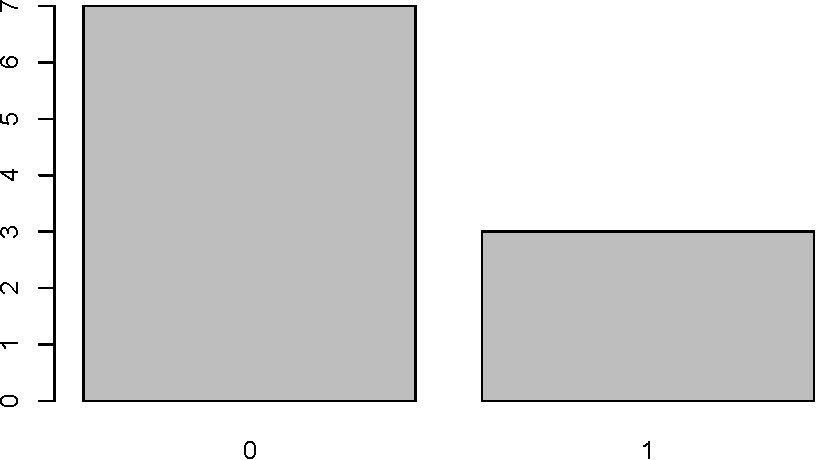
\includegraphics[width=0.9\linewidth]{bookdown_files/figure-latex/coinToss-1} \caption{Summary bar plot of coin tosses.}\label{fig:coinToss}
\end{figure}

Running these lines of code in a script window causes this plot to appear automatically under the Plots tab in the lower right RStudio window. We can save the plot image or copy and paste it into a report using menu option Export under the Plots tab. Examining the plot shows the unusual result of seven ``tails'' and three ``heads''. We would expect the counts to be about equal for the two categories, given the assumed probability of success (p) for a fair coin of 0.5.

Can you think of a physical process (hands-on method) that would produce Bernoulli data using other values for p, such as 0.25 or 0.33? What value for p might you expect for a fisheries examples, such as an annual exploitation rate (probability of being harvested), tag reporting rate (probability of angler returning a tag), or survival rate of adult fish in a lake (probability of surviving from year i to i+1)? These are the kinds of parameters that a field biologist might need to estimate. In the chapters that follow, we will examine some methods for collecting the data and estimating those probabilities.

We can generate simulated observations from a Bernoulli distribution using the \texttt{rbinom()} function:

\begin{Shaded}
\begin{Highlighting}[]
\NormalTok{N.obs }\OtherTok{\textless{}{-}} \DecValTok{30}
\NormalTok{p }\OtherTok{\textless{}{-}} \FloatTok{0.4}
\NormalTok{y }\OtherTok{\textless{}{-}} \FunctionTok{rbinom}\NormalTok{(}\AttributeTok{n=}\NormalTok{N.obs, }\AttributeTok{prob=}\NormalTok{p, }\AttributeTok{size=}\DecValTok{1}\NormalTok{)}
\NormalTok{Counts }\OtherTok{\textless{}{-}} \FunctionTok{table}\NormalTok{(y)  }\CommentTok{\# Summary table of 0 vs 1}
\FunctionTok{barplot}\NormalTok{(Counts)}
\end{Highlighting}
\end{Shaded}

The \texttt{rbinom()} function generates values from a binomial distribution (described in Section \ref{BinomialDist}). If we set the trial size to 1 (e.g., a single coin toss), we simulate draws from a Bernoulli distribution. The other two arguments in the \texttt{rbinom()} function are how many Bernoulli trials to simulate (n) and the probability of success (prob). How many values of 1 would you expect the vector y to contain in a vector of 30 replicate observations? As above, the final two lines can be used to count 0s and 1s and view a plot for these simulated data.

One of the most important benefits of using simulation is the ability to examine results from large sample sizes. For example, the following code shows that the \texttt{rbinom()} function produces an outcome very close to the expected proportion of 0s and 1s:

\begin{Shaded}
\begin{Highlighting}[]
\FunctionTok{rm}\NormalTok{(}\AttributeTok{list=}\FunctionTok{ls}\NormalTok{()) }\CommentTok{\# Clear Environment}

\NormalTok{N.obs }\OtherTok{\textless{}{-}} \DecValTok{1000}
\NormalTok{p }\OtherTok{\textless{}{-}} \FloatTok{0.4}
\NormalTok{y }\OtherTok{\textless{}{-}} \FunctionTok{rbinom}\NormalTok{(}\AttributeTok{n=}\NormalTok{N.obs, }\AttributeTok{prob=}\NormalTok{p, }\AttributeTok{size=}\DecValTok{1}\NormalTok{)}
\NormalTok{SumOnes }\OtherTok{\textless{}{-}} \FunctionTok{sum}\NormalTok{(y)}
\NormalTok{SumOnes}
\NormalTok{SumOnes}\SpecialCharTok{/}\NormalTok{N.obs }\CommentTok{\# Proportion of trials that are successful}
\NormalTok{Counts }\OtherTok{\textless{}{-}} \FunctionTok{table}\NormalTok{(y)}
\FunctionTok{barplot}\NormalTok{(Counts)}
\end{Highlighting}
\end{Shaded}

The first line of code just clears the Environment, ensuring that we start from a clean slate. The \texttt{sum()} function provides a total for the y vector, which is equal to the number of successful trials. Dividing by the number of observations is an empirical estimate of p.~The plot (Plot window) shows the result for one simulation (with N.obs replicates). How close to the expected count of 1s (400) did you observe? How much does the result vary when you do multiple simulations? (Highlight all the statements and click Run several times to see the variation.)

\hypertarget{BinomialDist}{%
\subsection{Binomial}\label{BinomialDist}}

The binomial distribution\index{Distribution, Binomial} is simply the combined total from multiple Bernoulli trials. One physical example would be the number of heads in five tosses of a coin. Each toss is an independent Bernoulli trial, but we record the total number of successes (heads). We could obtain anything between 0 and 5 heads in a single trial. We assume that the probability of success (p) is constant for each Bernoulli trial (e.g., each coin toss).

One fisheries example of a binomially distributed process would be the number of recaptures in a two-sample mark-recapture study. In that case, the number of fish in the second sample is the size of the trial, and fraction of the population that is marked is the probability p.~Another fisheries example would be the number of tag returns in a study to estimate the exploitation rate (rate of harvest). The number of tagged fish is the size of the trial and the exploitation rate is p.~A telemetry study to estimate fish survival rate is a third example. The initial number of fish with transmitters is the size of the trial. The survival rate is p and the number of survivors at the start of the next period is binomially distributed.

Let's start with a physical example of drawing five playing cards (with replacement) and recording the number of clubs. The probability of success in this case (drawing a club) is 0.25 and there are six possible outcomes (0-5 clubs). The expected number of clubs is 1.25 (trial size * p).

\begin{Shaded}
\begin{Highlighting}[]
\FunctionTok{rm}\NormalTok{(}\AttributeTok{list=}\FunctionTok{ls}\NormalTok{()) }\CommentTok{\# Clear Environment}

\NormalTok{Clubs }\OtherTok{\textless{}{-}}\FunctionTok{c}\NormalTok{(}\DecValTok{0}\NormalTok{, }\DecValTok{0}\NormalTok{, }\DecValTok{3}\NormalTok{, }\DecValTok{3}\NormalTok{, }\DecValTok{1}\NormalTok{, }\DecValTok{1}\NormalTok{)  }\CommentTok{\# Drawing five cards, with replacement}
\NormalTok{N.trials }\OtherTok{\textless{}{-}} \FunctionTok{length}\NormalTok{(Clubs) }\CommentTok{\# Function for getting number of trials}
\NormalTok{Counts }\OtherTok{\textless{}{-}} \FunctionTok{table}\NormalTok{(Clubs)}
\FunctionTok{barplot}\NormalTok{(Counts)}
\FunctionTok{barplot}\NormalTok{(Counts, }\AttributeTok{xlab=}\StringTok{"Number of clubs"}\NormalTok{)}
\end{Highlighting}
\end{Shaded}

Again we let R count the number of trials (6 in this case) and use the \texttt{table()} function to summarize the outcomes. Our sample size is small and the plot only shows the three observed outcomes. The plot can be made more understandable (especially by someone else) by adding a plot option (xlab) to label the x axis. Doing more than one plot produces a sequence of plots which you can view by using the blue left and right arrows in the Plot window. Practice modifying the above code by adding a label for the y axis (e.g., ``Frequency''). You can find the full list of bar plot options by entering ``barplot'' in the search box in the RStudio help window (or simply type ?barplot) in the Console).

We can alleviate our small sample size issue by turning to a simulation version. We again use the \texttt{rbinom()} function from the Bernoulli example, but now size is greater than 1:

\begin{Shaded}
\begin{Highlighting}[]
\FunctionTok{rm}\NormalTok{(}\AttributeTok{list=}\FunctionTok{ls}\NormalTok{()) }\CommentTok{\# Clear Environment}

\NormalTok{N.trials }\OtherTok{\textless{}{-}} \DecValTok{30}
\NormalTok{p }\OtherTok{\textless{}{-}} \FloatTok{0.25} \CommentTok{\# Probability of drawing a club}
\NormalTok{Trial.size }\OtherTok{\textless{}{-}} \DecValTok{5}
\NormalTok{Clubs }\OtherTok{\textless{}{-}} \FunctionTok{rbinom}\NormalTok{(}\AttributeTok{n=}\NormalTok{N.trials, }\AttributeTok{prob=}\NormalTok{p, }\AttributeTok{size=}\NormalTok{Trial.size)}
\NormalTok{Clubs}
\NormalTok{Counts }\OtherTok{\textless{}{-}} \FunctionTok{table}\NormalTok{(Clubs)}
\FunctionTok{barplot}\NormalTok{(Counts)}
\end{Highlighting}
\end{Shaded}

Each of the thirty observations now represents a trial size of 5 (in total, a simulation equivalent to 150 Bernoulli trials). Only part of the Clubs vector is visible in the Environment window but we can put Clubs as a line of code to print the whole vector in the Console. We again summarize the counts and plot the results using the \texttt{barplot()} function. Highlight the code in the Source window and run it multiple times to get some insight into the variability of the simulated system. For example, how often do you observe 0 or 5 Clubs? Which outcome(s) occurs most often (mode) and how frequently does the mode change?

We would expect to observe very few trials with 5 successes, because the probability is quite low (0.25\textsuperscript{5}=0.001). We can calculate it in the Console, by entering the expression 0.25\^{}5. There is a higher probability of 0 successes (0.24), which can be calculated as 0.75\^{}5 or (1-p)\textsuperscript{5}, because 1-p is the probability of failure (not getting a club). It is more involved to calculate the probabilities of 1-4 successes because they can be obtained multiple ways (e.g., 1 success can be obtained five ways (10000, 01000, 00100, 00010, 00001). We could calculate those probabilities using the binomial probability distribution: \(f(k) = {n \choose k} p^{k} (1-p)^{n-k}\), where k is the number of successes in a trial of size n.~R code for this calculation uses the \texttt{choose()} function; for example, \texttt{choose(Trial.size,0)\ *\ p\^{}0\ *\ (1-p)\^{}5} calculates the probability of 0 clubs in five draws. We could get an approximate (``brute force'') estimate of the probabilities by increasing N.trials to a large value (say 10,000) and dividing the Counts vector by N.trials to estimate at the proportion of trials resulting in 0, 1,\ldots5 successes:

\begin{Shaded}
\begin{Highlighting}[]
\FunctionTok{rm}\NormalTok{(}\AttributeTok{list=}\FunctionTok{ls}\NormalTok{()) }\CommentTok{\# Clear Environment}

\NormalTok{N.trials }\OtherTok{\textless{}{-}} \DecValTok{10000}
\NormalTok{p }\OtherTok{\textless{}{-}} \FloatTok{0.25} \CommentTok{\# Probability of drawing a club}
\NormalTok{Trial.size }\OtherTok{\textless{}{-}} \DecValTok{5}
\NormalTok{Clubs }\OtherTok{\textless{}{-}} \FunctionTok{rbinom}\NormalTok{(}\AttributeTok{n=}\NormalTok{N.trials, }\AttributeTok{prob=}\NormalTok{p, }\AttributeTok{size=}\NormalTok{Trial.size)}
\CommentTok{\#Clubs}
\NormalTok{Counts }\OtherTok{\textless{}{-}} \FunctionTok{table}\NormalTok{(Clubs)}
\FunctionTok{barplot}\NormalTok{(Counts)}
\NormalTok{Counts}\SpecialCharTok{/}\NormalTok{N.trials }\CommentTok{\# Vector division {-} probabilities of 0{-}5 Clubs}
\end{Highlighting}
\end{Shaded}

Note that we used a pound sign to turn off (``comment out'') the line for printing the Clubs vector to the Console, and print to the Console the estimated probabilities. The mode of our simulated distribution is in agreement with the expected value (trial size * p), as are the estimated probabilities for 0 and 5 clubs.

\hypertarget{Multinomial}{%
\subsection{Multinomial}\label{Multinomial}}

The Bernoulli and binomial distributions return a single value: success or failure for the Bernoulli and the number of successes (out of a specified trial size) for the binomial. The multinomial distribution\index{Distribution, Multinomial} extends that to a vector of results. A classic physical example would be to roll a die several times and record how many rolls were a 1, 2, \ldots, 6. A fisheries example would be to collect a sample of fish and determine how many are age 1, 2,\ldots{} The focus in that example is on estimating the age distribution, or proportions of fish by age. An age distribution contains valuable information about the rates of mortality and recruitment (year-class strength). Another fisheries example would be to collect a sample of fish (e.g., from electrofishing or a trawl) and determine the number caught by species. Species composition can be an important indicator of the ecological health of a study site (e.g.~if there is a high relative abundance of species considered tolerant of poor water quality).

Let's begin with a hands-on example. I roll a die ten times, and record as a vector the number of times I get a 1, 2, \ldots, 6:

\begin{Shaded}
\begin{Highlighting}[]
\FunctionTok{rm}\NormalTok{(}\AttributeTok{list=}\FunctionTok{ls}\NormalTok{()) }\CommentTok{\# Clear Environment}

\NormalTok{x }\OtherTok{\textless{}{-}}\FunctionTok{c}\NormalTok{(}\DecValTok{2}\NormalTok{,}\DecValTok{3}\NormalTok{,}\DecValTok{3}\NormalTok{,}\DecValTok{0}\NormalTok{,}\DecValTok{2}\NormalTok{,}\DecValTok{0}\NormalTok{)  }\CommentTok{\# Generated using die, equal cell probabilities}
\NormalTok{SampleSize }\OtherTok{\textless{}{-}} \FunctionTok{sum}\NormalTok{(x)}
\FunctionTok{barplot}\NormalTok{(x)}
\end{Highlighting}
\end{Shaded}

Here R calculates the sample size (SampleSize), even though we know in this instance that there were 10 rolls. The \texttt{barplot()} function generates the plot but without any labels is not very appealing. We can dress it up a bit by adding some options (Figure \ref{fig:dieRoll}). We first create a vector with values 1-6 to serve as x-axis labels (\texttt{seq()} function, from 1 to 6 by 1). Then we use the names.arg option to add the labels, and add x and y axis titles using xlab and ylab respectively.

\begin{Shaded}
\begin{Highlighting}[]
\NormalTok{x.labels }\OtherTok{\textless{}{-}} \FunctionTok{seq}\NormalTok{(}\AttributeTok{from=}\DecValTok{1}\NormalTok{, }\AttributeTok{to=}\DecValTok{6}\NormalTok{, }\AttributeTok{by=}\DecValTok{1}\NormalTok{)  }\CommentTok{\# x axis labels for plotting}
\FunctionTok{barplot}\NormalTok{(x, }\AttributeTok{names.arg=}\NormalTok{x.labels, }\AttributeTok{xlab=}\StringTok{"Die side"}\NormalTok{, }\AttributeTok{ylab=}\StringTok{"Number of rolls"}\NormalTok{)}
\end{Highlighting}
\end{Shaded}

\begin{figure}
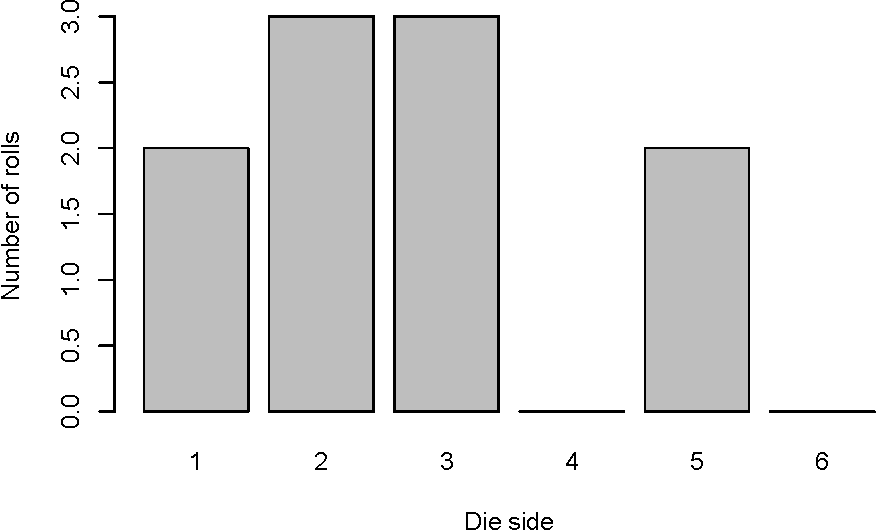
\includegraphics[width=0.9\linewidth]{bookdown_files/figure-latex/dieRoll-1} \caption{Summary bar plot of die rolls.}\label{fig:dieRoll}
\end{figure}

We can simulate a multinomial distribution as follows:

\begin{Shaded}
\begin{Highlighting}[]
\FunctionTok{rm}\NormalTok{(}\AttributeTok{list=}\FunctionTok{ls}\NormalTok{()) }\CommentTok{\# Clear Environment}

\NormalTok{SampleSize }\OtherTok{\textless{}{-}} \DecValTok{30}  \CommentTok{\# e.g., sample of 30 fish assigned by age}
\NormalTok{TrueP }\OtherTok{\textless{}{-}} \FunctionTok{c}\NormalTok{(}\FloatTok{0.1}\NormalTok{, }\FloatTok{0.3}\NormalTok{, }\FloatTok{0.4}\NormalTok{, }\FloatTok{0.1}\NormalTok{, }\FloatTok{0.05}\NormalTok{, }\FloatTok{0.05}\NormalTok{) }\CommentTok{\# probability of being ages 1{-}6}
\NormalTok{Reps }\OtherTok{\textless{}{-}} \DecValTok{1} \CommentTok{\# How many replicate multinomial trials to carry out}

\CommentTok{\# Simulate a single trial using rmultinom function}
\FunctionTok{rmultinom}\NormalTok{(}\AttributeTok{n=}\NormalTok{Reps, }\AttributeTok{prob=}\NormalTok{TrueP, }\AttributeTok{size=}\NormalTok{SampleSize) }\CommentTok{\# Prints matrix to Console}
\NormalTok{x }\OtherTok{\textless{}{-}} \FunctionTok{rmultinom}\NormalTok{(}\AttributeTok{n=}\NormalTok{Reps, }\AttributeTok{prob=}\NormalTok{TrueP, }\AttributeTok{size=}\NormalTok{SampleSize)}
\CommentTok{\# x contains matrix of counts (one column per Rep)}
\NormalTok{x.vec }\OtherTok{\textless{}{-}} \FunctionTok{as.vector}\NormalTok{(}\FunctionTok{t}\NormalTok{(x)) }\CommentTok{\# Transpose matrix then convert to vector}

\NormalTok{age.vec }\OtherTok{\textless{}{-}} \FunctionTok{seq}\NormalTok{(}\DecValTok{1}\NormalTok{,}\DecValTok{6}\NormalTok{, }\AttributeTok{by=}\DecValTok{1}\NormalTok{)}
\FunctionTok{barplot}\NormalTok{(x.vec, }\AttributeTok{names.arg=}\NormalTok{age.vec, }\AttributeTok{xlab=}\StringTok{"Age"}\NormalTok{, }\AttributeTok{ylab=}\StringTok{"Number of fish"}\NormalTok{)}
\end{Highlighting}
\end{Shaded}

In this simulation, the age proportions (TrueP) are arbitrarily chosen (but could be based on field data). Run statements one-by-one to see how each line of code works. Note that the \texttt{rmultinom()} function returns a matrix with six rows and one column (n determines how many columns are returned). Rather than a column, we want a row vector, with the number of fish by age in successive columns. We use the \texttt{t()} (transpose) function to transpose the matrix and the \texttt{as.vector()} function to convert the matrix (with one row) into a row vector. We could have done this transformation in two steps but instead have nested the two functions. That results in more compact code but it is always a fine option to do the steps separately for greater clarity.

Run the code beginning with the \texttt{x\ \textless{}-\ rmultinom()} line several times to see how much the age distribution varies from one random sample to the next. The underlying age proportions are fixed, but the counts vary quite a bit for this small sample size. This is an example of how simulation is helpful in gaining experience and intuition in judging pure sampling variation versus a real biological result (e.g.~good or bad year-class strength).

\hypertarget{poisson}{%
\subsection{Poisson}\label{poisson}}

Like the Bernoulli, binomial, and multinomial distributions, the Poisson\index{Distribution, Poisson} and negative binomial distributions are used for counts (non-negative whole numbers). The first three cases have an upper bound (1 for the Bernoulli, trial size for the next two) whereas the Poisson and negative binomial distributions do not (in theory, if not in practical terms). The Poisson is simpler than the negative binomial in that it is described by a single parameter, usually \(\lambda\), which represents the mean and variance of the distribution. A fisheries example of a Poisson distribution could be the number of fish per day moving upstream via a fish ladder. A model for this process could be useful for designing new fish ladders to have an appropriate capacity. Another example could be the number of fish caught per trawl tow. In this case, emphasis might be placed on how trawl catches vary from year to year, as an indication of population status.

Our simulation uses an arbitrary value for \(\lambda\):

\begin{Shaded}
\begin{Highlighting}[]
\FunctionTok{rm}\NormalTok{(}\AttributeTok{list=}\FunctionTok{ls}\NormalTok{()) }\CommentTok{\# Clear Environment}

\NormalTok{N }\OtherTok{\textless{}{-}} \DecValTok{30}
\NormalTok{lambda }\OtherTok{\textless{}{-}} \DecValTok{4}
\NormalTok{Count }\OtherTok{\textless{}{-}} \FunctionTok{rpois}\NormalTok{(}\AttributeTok{n=}\NormalTok{N, }\AttributeTok{lambda=}\NormalTok{lambda)}
\NormalTok{Freq }\OtherTok{\textless{}{-}} \FunctionTok{table}\NormalTok{(Count)  }\CommentTok{\# Distribution of simulated counts}
\FunctionTok{barplot}\NormalTok{(Freq, }\AttributeTok{main=}\StringTok{""}\NormalTok{, }\AttributeTok{xlab=}\StringTok{"Count"}\NormalTok{, }\AttributeTok{ylab=}\StringTok{"Frequency"}\NormalTok{)}

\FunctionTok{mean}\NormalTok{(Count)}
\FunctionTok{var}\NormalTok{(Count)}
\end{Highlighting}
\end{Shaded}

Run the lines of code multiple times to gain experience with the Poisson distribution. How often is the mode of the distribution equal to \(\lambda\)? Are the estimated mean and variance (printed to the Console) close to \(\lambda\)? Increase the sample size to get a smooth distribution and reliable estimates of the two sample statistics.

It is also useful to run the code using other values for \(\lambda\). What value for \(\lambda\) causes the mode to shift to 0? At what value does the sample distribution look like a bell curve (i.e., symmetrical)? One of the key benefits of simulation is that we can easily try different scenarios to build understanding about the system being modeled.

The plot can sometimes be misleading because it only includes observed levels. We can modify the code to include levels with a frequency of zero:

\begin{Shaded}
\begin{Highlighting}[]
\FunctionTok{rm}\NormalTok{(}\AttributeTok{list=}\FunctionTok{ls}\NormalTok{()) }\CommentTok{\# Clear Environment}

\NormalTok{N }\OtherTok{\textless{}{-}} \DecValTok{30}
\NormalTok{lambda }\OtherTok{\textless{}{-}} \DecValTok{4}
\NormalTok{Count }\OtherTok{\textless{}{-}} \FunctionTok{rpois}\NormalTok{(}\AttributeTok{n=}\NormalTok{N, }\AttributeTok{lambda=}\NormalTok{lambda) }\CommentTok{\# Counts drawn from Poisson distribution}
\NormalTok{Freq }\OtherTok{\textless{}{-}} \FunctionTok{table}\NormalTok{(}\FunctionTok{factor}\NormalTok{(Count, }\AttributeTok{levels =} \DecValTok{0}\SpecialCharTok{:}\FunctionTok{max}\NormalTok{(Count)))}
\FunctionTok{barplot}\NormalTok{(Freq, }\AttributeTok{main=}\StringTok{""}\NormalTok{, }\AttributeTok{xlab=}\StringTok{"Count"}\NormalTok{, }\AttributeTok{ylab=}\StringTok{"Frequency"}\NormalTok{)}

\FunctionTok{mean}\NormalTok{(Count)}
\FunctionTok{var}\NormalTok{(Count)}
\end{Highlighting}
\end{Shaded}

Now the \texttt{table()} function operates on counts transformed into factors (categories or levels) by the \texttt{factor()} function. The levels= argument forces \texttt{factor()} to use a range of levels from 0 to \texttt{max(Count)}, in order to include levels with a frequency of zero. Try the following partial code in the Console to see the levels (``0'', ``1'', etc) created by the \texttt{factor()} function: \texttt{myfact\ \textless{}-\ factor(Count,\ levels\ =\ 0:max(Count))}.

\hypertarget{negative-binomial}{%
\subsection{Negative binomial}\label{negative-binomial}}

As noted above, the negative binomial\index{Distribution, Negative Binomial} distribution is used in similar situations to the Poisson except that it has two parameters and is therefore more flexible. This is particularly helpful for ecological data, where counts are often more variable than would be expected under a Poisson distribution \citep{bolker2008, link.barker_2009}. The R function for generating negative binomial random variates (\texttt{rnbinom()}) can be parameterized in different ways; we use the ``ecological'' parameterization recommended by \citet{bolker2008}. This uses the mean (termed \(\mu\)) but not the variance, instead using an overdispersion parameter k. Lower values of k result in a more heterogeneous distribution, and in ecological settings, k is often less than the mean \citep{bolker2008}. The distribution approximates a Poisson when k is large. The code includes calculation of the variance as a function of mu and k \citep{bolker2008}. Alternatively the mean and variance (V) can be specified and used to solve for k: \(k = \mu^2/(V-\mu)\).

\begin{Shaded}
\begin{Highlighting}[]
\FunctionTok{rm}\NormalTok{(}\AttributeTok{list=}\FunctionTok{ls}\NormalTok{()) }\CommentTok{\# Clear Environment}

\NormalTok{N }\OtherTok{\textless{}{-}} \DecValTok{30}
\NormalTok{mu }\OtherTok{\textless{}{-}} \DecValTok{4}
\NormalTok{k}\OtherTok{=}\DecValTok{1}
\NormalTok{variance }\OtherTok{\textless{}{-}}\NormalTok{ mu}\SpecialCharTok{+}\NormalTok{(mu}\SpecialCharTok{\^{}}\DecValTok{2}\NormalTok{)}\SpecialCharTok{/}\NormalTok{k}
\NormalTok{Count }\OtherTok{\textless{}{-}} \FunctionTok{rnbinom}\NormalTok{(}\AttributeTok{n=}\NormalTok{N, }\AttributeTok{mu=}\NormalTok{mu, }\AttributeTok{size=}\NormalTok{k)}
\NormalTok{Freq }\OtherTok{\textless{}{-}} \FunctionTok{table}\NormalTok{(}\FunctionTok{factor}\NormalTok{(Count, }\AttributeTok{levels =} \DecValTok{0}\SpecialCharTok{:}\FunctionTok{max}\NormalTok{(Count)))}
\FunctionTok{barplot}\NormalTok{(Freq, }\AttributeTok{main=}\StringTok{""}\NormalTok{, }\AttributeTok{xlab=}\StringTok{"Count"}\NormalTok{, }\AttributeTok{ylab=}\StringTok{"Frequency"}\NormalTok{)}

\FunctionTok{mean}\NormalTok{(Count)}
\FunctionTok{var}\NormalTok{(Count)}
\end{Highlighting}
\end{Shaded}

This distribution has the same mean as in the Poisson example but tends to have a longer tail (occasional large counts). Rerun the code using different values for k; for example, Figure \ref{fig:NB-vary-k} uses a sample size of 200 to compare results for k=1 and k=10, each with \(\mu\)=4.

\begin{Shaded}
\begin{Highlighting}[]
\NormalTok{N }\OtherTok{\textless{}{-}} \DecValTok{200}
\NormalTok{mu }\OtherTok{\textless{}{-}} \DecValTok{4}
\NormalTok{k}\OtherTok{=}\DecValTok{1}
\NormalTok{Count }\OtherTok{\textless{}{-}} \FunctionTok{rnbinom}\NormalTok{(}\AttributeTok{n=}\NormalTok{N, }\AttributeTok{mu=}\NormalTok{mu, }\AttributeTok{size=}\NormalTok{k)}
\NormalTok{Freq }\OtherTok{\textless{}{-}} \FunctionTok{table}\NormalTok{(}\FunctionTok{factor}\NormalTok{(Count, }\AttributeTok{levels =} \DecValTok{0}\SpecialCharTok{:}\FunctionTok{max}\NormalTok{(Count)))}
\FunctionTok{barplot}\NormalTok{(Freq, }\AttributeTok{main=}\StringTok{""}\NormalTok{, }\AttributeTok{xlab=}\StringTok{"Count"}\NormalTok{, }\AttributeTok{ylab=}\StringTok{"Frequency"}\NormalTok{)}

\NormalTok{k}\OtherTok{=}\DecValTok{10} \CommentTok{\# Reduce degree of overdispersion}
\NormalTok{Count }\OtherTok{\textless{}{-}} \FunctionTok{rnbinom}\NormalTok{(}\AttributeTok{n=}\NormalTok{N, }\AttributeTok{mu=}\NormalTok{mu, }\AttributeTok{size=}\NormalTok{k)}
\NormalTok{Freq }\OtherTok{\textless{}{-}} \FunctionTok{table}\NormalTok{(}\FunctionTok{factor}\NormalTok{(Count, }\AttributeTok{levels =} \DecValTok{0}\SpecialCharTok{:}\FunctionTok{max}\NormalTok{(Count)))}
\FunctionTok{barplot}\NormalTok{(Freq, }\AttributeTok{main=}\StringTok{""}\NormalTok{, }\AttributeTok{xlab=}\StringTok{"Count"}\NormalTok{, }\AttributeTok{ylab=}\StringTok{"Frequency"}\NormalTok{)}
\end{Highlighting}
\end{Shaded}

\begin{figure}
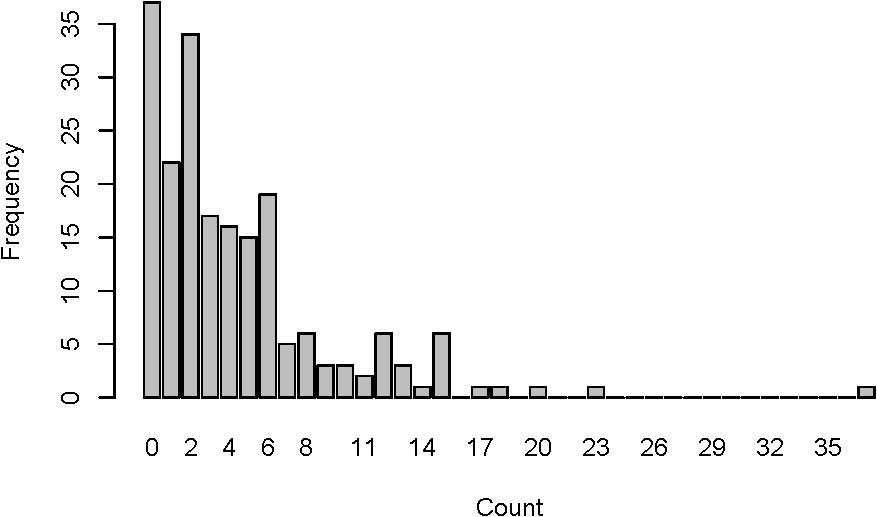
\includegraphics[width=0.5\linewidth]{bookdown_files/figure-latex/NB-vary-k-1} 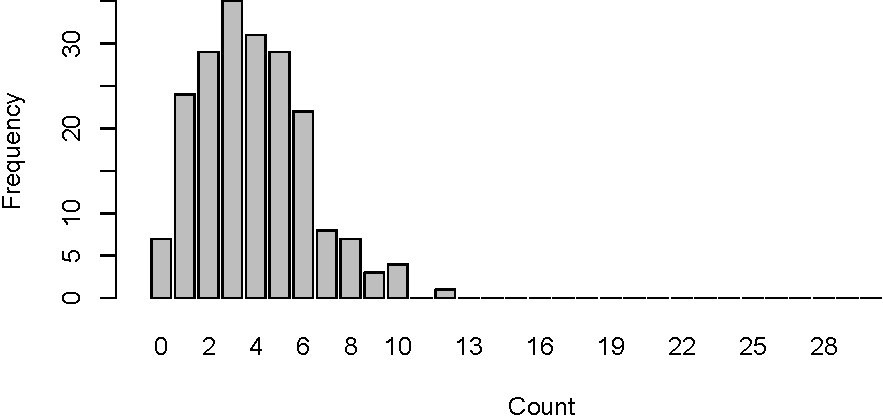
\includegraphics[width=0.5\linewidth]{bookdown_files/figure-latex/NB-vary-k-2} \caption{Negative binomial frequency distributions for k=1 (left) and 10 (right).}\label{fig:NB-vary-k}
\end{figure}

\hypertarget{Continuous}{%
\section{Continuous}\label{Continuous}}

\hypertarget{Uniform}{%
\subsection{Uniform}\label{Uniform}}

A uniform distribution\index{Distribution, Uniform} (bounds a, b) is flat in shape, indicating that all values between a lower and upper bound are considered equally likely. It is also useful as a ``first'' model for situations where relatively little is known other than the lower and upper bounds \citep{law.kelton_1982}. Probabilities have default bounds of 0 and 1, so a fish population model might use a uniform 0-1 distribution for probabilities such as survival rate. More narrow bounds could be used in cases where prior information was available; for example, a pilot study might indicate that the tag-reporting rate would be expected to vary between 0.4 and 0.6. Another fisheries example would be a uniform distribution between 60 and 70, for simulating individual variation in maximum size for a growth curve.

We begin with a simulation example, using the default range of 0-1 for the \texttt{runif()} function:

\begin{Shaded}
\begin{Highlighting}[]
\FunctionTok{rm}\NormalTok{(}\AttributeTok{list=}\FunctionTok{ls}\NormalTok{()) }\CommentTok{\# Clear Environment}

\NormalTok{Reps }\OtherTok{\textless{}{-}} \DecValTok{30} \CommentTok{\# Replicate draws from a uniform distribution}
\NormalTok{p }\OtherTok{\textless{}{-}} \FunctionTok{runif}\NormalTok{(}\AttributeTok{n=}\NormalTok{Reps)}\CommentTok{\# Default range of 0{-}1. Can specify using min, max}
\FunctionTok{hist}\NormalTok{(p, }\AttributeTok{breaks=}\DecValTok{5}\NormalTok{, }\AttributeTok{main=}\StringTok{""}\NormalTok{)}
\end{Highlighting}
\end{Shaded}

Try running the code several times and note the variation in pattern from one simulation run to the next. We use the breaks=5 option in the \texttt{hist()} function so that the histogram bin intervals are stable among runs. Specifying a null character string for ``main='' prevents the plot from including a main title. Next, increase the sample size and note the increased smoothness of the observed distribution. What would be the expected mean of the distribution? Estimate the mean and compare the observed and expected value among runs.

As noted above, the \texttt{runif()} function allows for a uniform distribution using any lower and upper bounds. For example, we might simulate uncertainty about an exploitation rate (fraction of the population that is harvested) by allowing randomly drawn values in a specified interval; for example, \texttt{runif(n=Reps,\ min=0.3,\ max=0.4)}. The \texttt{runif()} function is not constrained to positive values; for example, it could be used with bounds -0.5 and 0.5 to simulate uncertainty about a parameter that is close to 0 but can be positive or negative. The chapters that follow will include many examples where a uniform distribution is relevant for fisheries modeling.

\hypertarget{beta}{%
\subsection{Beta}\label{beta}}

The beta distribution\index{Distribution, Beta} has a lower bound of 0 and an upper bound of 1, so it is useful for modeling parameters with those bounds (i.e., probabilities). A fisheries model might use a beta distribution to simulate variation in a survival probability or the probability of a tag being returned. The uniform distribution (Section \ref{Uniform}) can also be used for probabilities, but only for the case where all values are equally likely. The beta distribution is more flexible and can not only be flat but also u-shaped, bell-shaped, or left- or right-skewed. Figure \ref{fig:Beta} shows sample distributions for shape parameters \(\alpha\)=1 and \(\beta\)=0.5, 1, and 5.

\begin{figure}
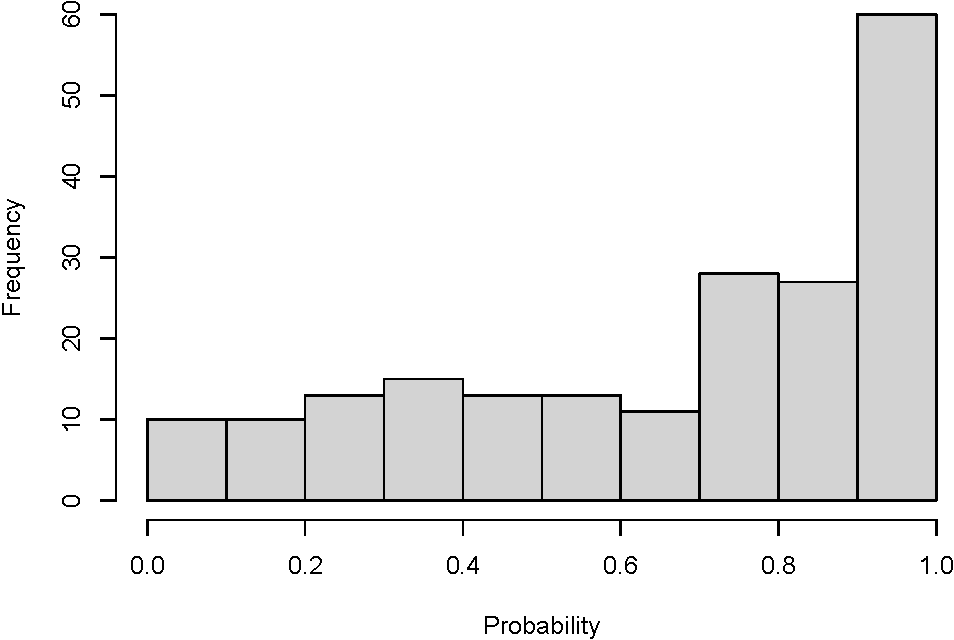
\includegraphics[width=0.33\linewidth]{bookdown_files/figure-latex/Beta-1} 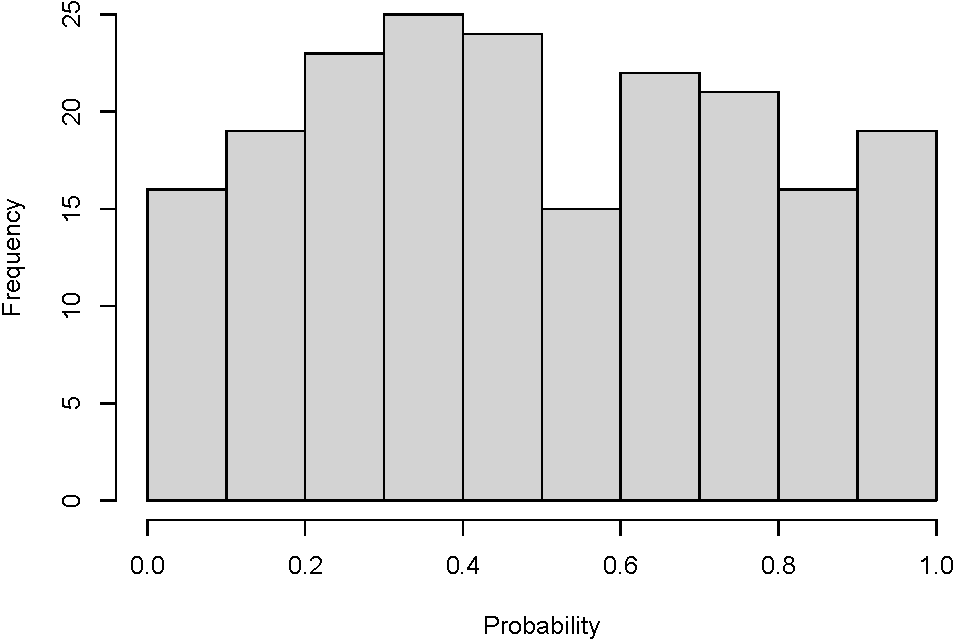
\includegraphics[width=0.33\linewidth]{bookdown_files/figure-latex/Beta-2} 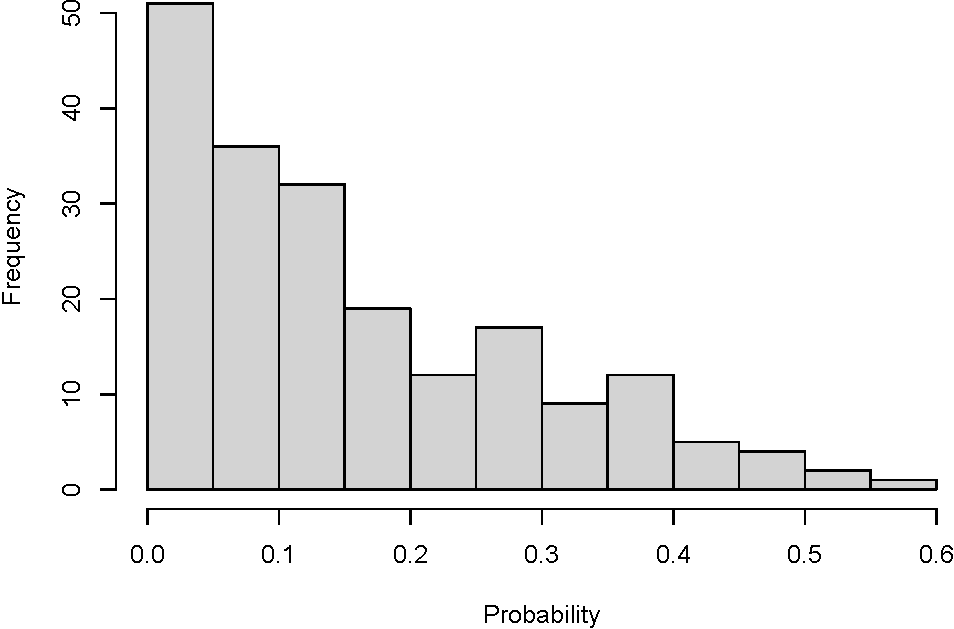
\includegraphics[width=0.33\linewidth]{bookdown_files/figure-latex/Beta-3} \caption{Histogram for 200 random draws from a beta distribution, with alpha=1 and beta=0.5  (left), 1 (center), and 5 (right).}\label{fig:Beta}
\end{figure}

We simulate draws from a beta distribution using the \texttt{rbeta()} function. Starting with \(\alpha\) and \(\beta\) set to 1 would be appropriate for a situation where all probabilities are equally likely:

\begin{Shaded}
\begin{Highlighting}[]
\FunctionTok{rm}\NormalTok{(}\AttributeTok{list=}\FunctionTok{ls}\NormalTok{()) }\CommentTok{\# Clear Environment}

\NormalTok{Reps }\OtherTok{\textless{}{-}} \DecValTok{200} \CommentTok{\# Replicate draws from a beta distribution}
\NormalTok{alpha }\OtherTok{\textless{}{-}} \DecValTok{1}
\NormalTok{beta }\OtherTok{\textless{}{-}} \DecValTok{1}
\NormalTok{x }\OtherTok{\textless{}{-}} \FunctionTok{rbeta}\NormalTok{(}\AttributeTok{n=}\NormalTok{Reps, }\AttributeTok{shape1=}\NormalTok{alpha, }\AttributeTok{shape2=}\NormalTok{beta)}
\FunctionTok{hist}\NormalTok{(x, }\AttributeTok{main=}\StringTok{""}\NormalTok{, }\AttributeTok{xlab=}\StringTok{"Probability"}\NormalTok{)}
\end{Highlighting}
\end{Shaded}

After running the above code multiple times, try a beta(8, 4) distribution. These parameter values could result from a pilot study with seven successes in ten trials (\(\alpha\)=7+1, \(\beta\)=3+1). This shifts the distribution toward a mode of 0.7, which is the observed proportion of successes in ten trials. Try other arbitrary values for the two parameters to vary the shape of the distribution. Can you think of a situation where probabilities would be expected to be close to 0 or close to 1?

\hypertarget{normal}{%
\subsection{Normal}\label{normal}}

The normal distribution\index{Distribution, Normal} is the well-known bell curve from traditional statistics courses. The distribution is unbounded (bounds -\(\infty\), \(\infty\)). The shape of the distribution is determined by the mean (location) and standard deviation (spread). A fisheries example might be a simulation where size-at-age varied among individuals according to a normal distribution.

Let's look at simulation code for length of individual fish, assuming a mean of 30 and standard deviation of 2:

\begin{Shaded}
\begin{Highlighting}[]
\FunctionTok{rm}\NormalTok{(}\AttributeTok{list=}\FunctionTok{ls}\NormalTok{()) }\CommentTok{\# Clear Environment}

\NormalTok{Reps }\OtherTok{\textless{}{-}} \DecValTok{30} \CommentTok{\# Replicate draws from a normal distribution}
\NormalTok{Len }\OtherTok{\textless{}{-}} \FunctionTok{rnorm}\NormalTok{(}\AttributeTok{n=}\NormalTok{Reps, }\AttributeTok{mean=}\DecValTok{30}\NormalTok{, }\AttributeTok{sd=}\DecValTok{2}\NormalTok{)}
\FunctionTok{hist}\NormalTok{(Len, }\AttributeTok{main=}\StringTok{""}\NormalTok{)}
\end{Highlighting}
\end{Shaded}

Run the code a few times to look at the variation in shape and bounds at a relatively small sample size. Next, increase the sample size and determine through trial and error the smallest sample size that provides a relatively smooth bell-curve shape. Estimate the mean and standard deviation (function \texttt{sd()}) and compare the observed and true values.

\hypertarget{lognormal}{%
\subsection{Lognormal}\label{lognormal}}

The lognormal distribution\index{Distribution, Lognormal} (bounds 0, \(\infty\)) is useful in ecological settings because it excludes negative values and allows for a long upper tail. A classic fisheries example of a lognormal distribution is annual recruitment for marine fish species (number of young entering the population). Most years result in low recruitment but there are occasional extreme values when environmental conditions are right.

We begin with simulation code:

\begin{Shaded}
\begin{Highlighting}[]
\FunctionTok{rm}\NormalTok{(}\AttributeTok{list=}\FunctionTok{ls}\NormalTok{()) }\CommentTok{\# Clear Environment}

\NormalTok{Reps }\OtherTok{\textless{}{-}} \DecValTok{200}
\NormalTok{ln.m }\OtherTok{\textless{}{-}} \DecValTok{0} \CommentTok{\# Ln{-}scale mean}
\NormalTok{ln.v }\OtherTok{\textless{}{-}} \FloatTok{0.5} \CommentTok{\# Ln{-}scale variance}
\NormalTok{y }\OtherTok{\textless{}{-}} \FunctionTok{rlnorm}\NormalTok{(}\AttributeTok{n=}\NormalTok{Reps, }\AttributeTok{mean=}\NormalTok{ln.m, }\AttributeTok{sd=}\FunctionTok{sqrt}\NormalTok{(ln.v))}

\FunctionTok{hist}\NormalTok{(y, }\AttributeTok{main=}\StringTok{"Lognormal distribution"}\NormalTok{)}
\NormalTok{Exp.mean }\OtherTok{\textless{}{-}} \FunctionTok{exp}\NormalTok{(ln.m}\SpecialCharTok{+}\NormalTok{(ln.v}\SpecialCharTok{/}\DecValTok{2}\NormalTok{)) }\CommentTok{\# Calculate arithmetic scale expected mean}
\FunctionTok{abline}\NormalTok{(}\AttributeTok{v=}\NormalTok{Exp.mean, }\AttributeTok{col=}\StringTok{"red"}\NormalTok{)}
\NormalTok{Exp.var }\OtherTok{\textless{}{-}}\NormalTok{ (}\FunctionTok{exp}\NormalTok{(}\DecValTok{2}\SpecialCharTok{*}\NormalTok{ln.m}\SpecialCharTok{+}\NormalTok{ln.v))}\SpecialCharTok{*}\NormalTok{(}\FunctionTok{exp}\NormalTok{(ln.v)}\SpecialCharTok{{-}}\DecValTok{1}\NormalTok{) }\CommentTok{\# Arithmetic scale expected variance}
\FunctionTok{mean}\NormalTok{(y)}
\FunctionTok{var}\NormalTok{(y)}
\end{Highlighting}
\end{Shaded}

The \texttt{rlnorm()} function generates random lognormal values, using an arbitrarily chosen mean and standard deviation specified in natural log-scale. Those values can be used to calculate the expected mean and variance in arithmetic scale. The \texttt{abline()} function can be used to add to the histogram a vertical (v=) line for the expected arithmetic-scale mean (Figure \ref{fig:Lognormal}). The line color is specified as col=``red''; other options including line weight and pattern can be found in the Help window. Compare the estimates of arithmetic-scale mean and variance for your (relatively large) sample of lognormal random variates to the expected values (visible in the Environment window).

\begin{figure}
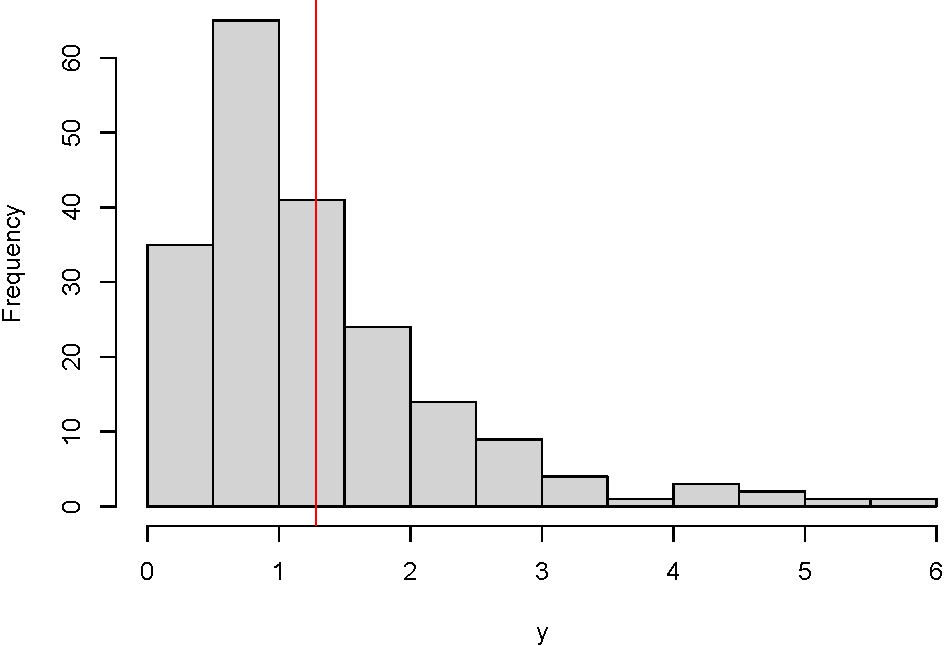
\includegraphics[width=0.9\linewidth]{bookdown_files/figure-latex/Lognormal-1} \caption{Histogram for 200 lognormally-distributed values, with ln-scale mean of 0 and variance of 0.5. Red vertical line denotes expected mean.}\label{fig:Lognormal}
\end{figure}

\hypertarget{gamma}{%
\subsection{Gamma}\label{gamma}}

The gamma distribution\index{Distribution, Gamma} is similar to the lognormal in that has a lower bound of 0 and an upper bound of \(\infty\). Thus it also excludes negative values and allows for a long upper tail. This distribution is often used to simulate waiting times (how long until some number of events has occurred, based on a specified average time between events). We consider it here simply because it can take on a variety of shapes depending on its parameters \citep{bolker2008}. Figure \ref{fig:Gamma} shows sample distributions for shape parameter \(\alpha\)=3 and scale or spread parameter \(\beta\)=1 and 3.

\begin{figure}
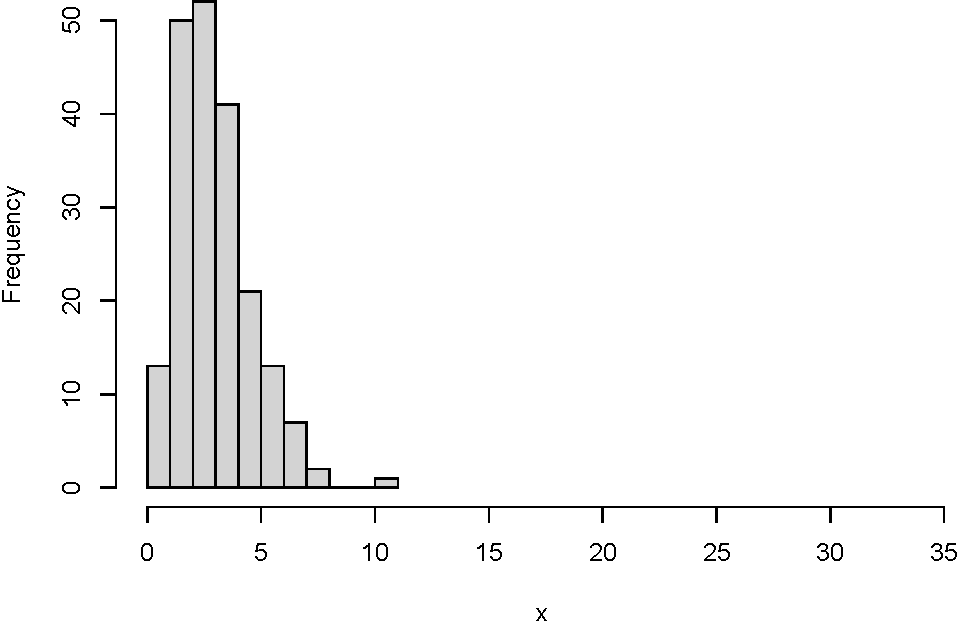
\includegraphics[width=0.5\linewidth]{bookdown_files/figure-latex/Gamma-1} 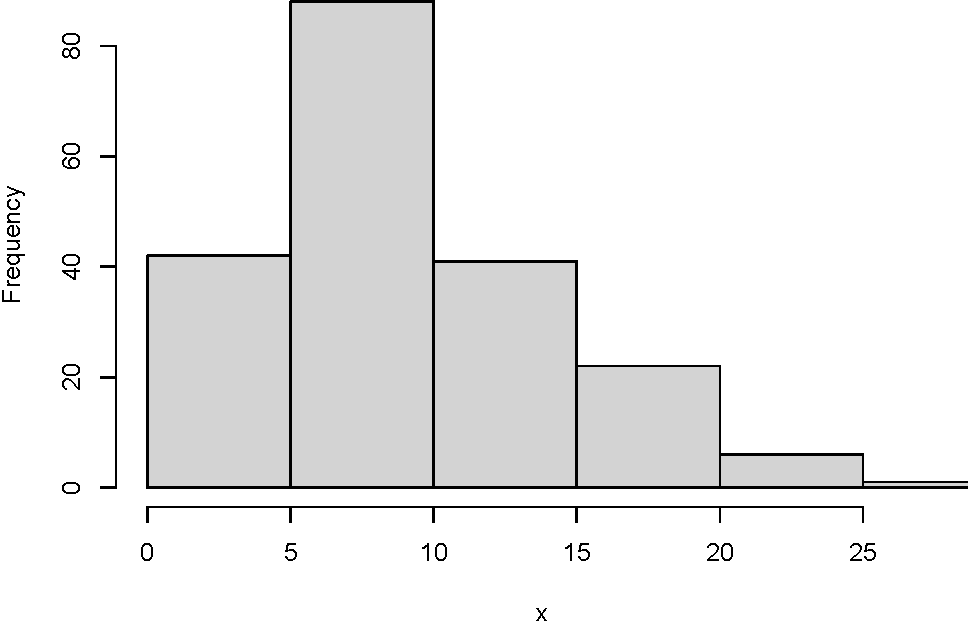
\includegraphics[width=0.5\linewidth]{bookdown_files/figure-latex/Gamma-2} \caption{Histogram for 200 gamma-distributed values, with alpha=3 and beta=1  (left) and 3 (right).}\label{fig:Gamma}
\end{figure}

We simulate draws from a gamma distribution using the \texttt{rgamma()} function, with arbitrary values for \(\alpha\) and \(\beta\):

\begin{Shaded}
\begin{Highlighting}[]
\FunctionTok{rm}\NormalTok{(}\AttributeTok{list=}\FunctionTok{ls}\NormalTok{()) }\CommentTok{\# Clear Environment}

\NormalTok{Reps }\OtherTok{\textless{}{-}} \DecValTok{200} \CommentTok{\# Replicate draws from a gamma distribution}
\NormalTok{alpha }\OtherTok{\textless{}{-}} \DecValTok{3} \CommentTok{\# Shape parameter, \textgreater{} 0}
\NormalTok{beta }\OtherTok{\textless{}{-}} \DecValTok{3} \CommentTok{\# Scale parameter, \textgreater{} 0}
\NormalTok{x }\OtherTok{\textless{}{-}} \FunctionTok{rgamma}\NormalTok{(}\AttributeTok{n=}\NormalTok{Reps, }\AttributeTok{shape=}\NormalTok{alpha, }\AttributeTok{scale=}\NormalTok{beta)}
\FunctionTok{hist}\NormalTok{(x, }\AttributeTok{main=}\StringTok{""}\NormalTok{)}
\NormalTok{Exp.mean }\OtherTok{\textless{}{-}}\NormalTok{ alpha}\SpecialCharTok{*}\NormalTok{beta}
\NormalTok{Exp.var }\OtherTok{\textless{}{-}}\NormalTok{ alpha}\SpecialCharTok{*}\NormalTok{beta}\SpecialCharTok{\^{}}\DecValTok{2}
\FunctionTok{mean}\NormalTok{(x)}
\FunctionTok{var}\NormalTok{(x)}
\end{Highlighting}
\end{Shaded}

A sample size of 200 replicates produces a relatively smooth pattern for the distribution. How close are the estimated mean and variance to the expected values for this sample size? Try adjusting the two parameters to vary the shape of the distribution. What values for \(\alpha\) and \(\beta\) produce a right-skewed distribution (long right tail), or a pattern somewhat like a normal distribution (bell-curve)?

\hypertarget{exercises}{%
\section{Exercises}\label{exercises}}

\begin{enumerate}
\def\labelenumi{\arabic{enumi}.}
\item
  Use a physical process (i.e., not simulated) to generate twenty Bernoulli observations with probability of success 0.25. Include in your code comments describing how you obtained the data. Produce a summary plot of the total number of 0s and 1s. How does your observed number of successes compare to what you would expect?
\item
  Use a physical process to generate ten binomially distributed observations, with a trial size of at least four. What is the probability of success and the expected number of successes per trial? Produce a histogram showing the frequencies for different numbers of success per trial.
\item
  Use a physical process to generate 10 outcomes from a multinomial process with at least three possible outcomes. Describe in your code comments the physical process for obtaining the data and include a plot of the frequencies. How do the frequencies compare to what you would expect?
\item
  Assume that the following vector contains trawl catches: y=c(7, 5, 1, 5, 0, 3, 8, 2, 14, 5, 0, 6, 9, 1, 2, 2, 1, 1, 0, 9, 2, 2, 4, 11, 1, 1, 7, 3, 1, 1). Based on your analysis (including plot), were these data likely generated from a Poisson or negative binomial distribution?
\item
  Provide simulation code for generating normally-distributed length data for fish ages 1 (n.1=40, age-1 mean 30, sd 5) and 2 (n.2=25, age-2 mean=50, sd=7). Plot the combined length sample. In multiple simulations using these default values, how frequently is the length distribution visibly bimodal?
\end{enumerate}

\cleardoublepage

\hypertarget{appendix-appendix}{%
\appendix \addcontentsline{toc}{chapter}{\appendixname}}


\hypertarget{title-placeholder}{%
\chapter{Title Placeholder}\label{title-placeholder}}

If there is anything to put in an appendix, it would go here.

  \bibliography{book.bib,packages.bib}

\backmatter
\printindex

\end{document}
